\documentclass[11pt,a4paper]{article}

% ── Packages ──────────────────────────────────────────────────────────
\usepackage[utf8]{inputenc}
\usepackage[T1]{fontenc}
\usepackage{lmodern}
\usepackage[margin=2.2cm]{geometry}
\usepackage{graphicx}
\usepackage{xcolor}
\usepackage{hyperref}
\usepackage{listings}
\usepackage{booktabs}
\usepackage{tabularx}
\usepackage{longtable}
\usepackage{enumitem}
\usepackage{fancyhdr}
\usepackage{titlesec}
\usepackage{tikz}
\usepackage{tcolorbox}
\usepackage{multicol}
\usepackage{float}

\usetikzlibrary{shapes.geometric, arrows.meta, positioning, fit, backgrounds, calc}

% ── Colors ────────────────────────────────────────────────────────────
\definecolor{primary}{HTML}{1B5E20}
\definecolor{accent}{HTML}{4CAF50}
\definecolor{darkbg}{HTML}{1E1E1E}
\definecolor{codebg}{HTML}{F5F5F5}
\definecolor{urlblue}{HTML}{1565C0}
\definecolor{warnred}{HTML}{C62828}
\definecolor{lockgold}{HTML}{F9A825}
\definecolor{publicgreen}{HTML}{2E7D32}

% ── Hyperref Setup ────────────────────────────────────────────────────
\hypersetup{
    colorlinks=true,
    linkcolor=primary,
    urlcolor=urlblue,
    citecolor=primary,
    pdftitle={KhetiMitra API Documentation},
    pdfauthor={KhetiMitra Engineering},
}

% ── Code Listings ─────────────────────────────────────────────────────
\lstdefinestyle{jsonStyle}{
    backgroundcolor=\color{codebg},
    basicstyle=\ttfamily\small,
    breaklines=true,
    frame=single,
    rulecolor=\color{black!20},
    xleftmargin=4pt,
    xrightmargin=4pt,
    aboveskip=8pt,
    belowskip=8pt,
    showstringspaces=false,
}
\lstdefinestyle{bashStyle}{
    backgroundcolor=\color{darkbg},
    basicstyle=\ttfamily\small\color{white},
    breaklines=true,
    frame=single,
    rulecolor=\color{black!40},
    xleftmargin=4pt,
    xrightmargin=4pt,
    aboveskip=8pt,
    belowskip=8pt,
    showstringspaces=false,
}

% ── tcolorbox Styles ──────────────────────────────────────────────────
\tcbuselibrary{skins, breakable}

\newtcolorbox{endpoint}[2][]{%
    colback=codebg, colframe=primary, fonttitle=\bfseries\ttfamily,
    title={#2}, breakable, left=4pt, right=4pt, top=4pt, bottom=4pt, #1
}

\newtcolorbox{infobox}[1][]{%
    colback=blue!5, colframe=urlblue!70, fonttitle=\bfseries,
    breakable, left=4pt, right=4pt, #1
}

\newtcolorbox{warnbox}[1][]{%
    colback=red!5, colframe=warnred!70, fonttitle=\bfseries,
    title={Important}, breakable, left=4pt, right=4pt, #1
}

% ── Headers & Footers ────────────────────────────────────────────────
\pagestyle{fancy}
\fancyhf{}
\fancyhead[L]{\small\textcolor{primary}{\textbf{KhetiMitra}} -- API Documentation}
\fancyhead[R]{\small v1.0}
\fancyfoot[C]{\thepage}
\renewcommand{\headrulewidth}{0.4pt}

% ── Section Formatting ───────────────────────────────────────────────
\titleformat{\section}
    {\Large\bfseries\color{primary}}{\thesection}{1em}{}[\vspace{2pt}\titlerule]
\titleformat{\subsection}
    {\large\bfseries\color{primary!80!black}}{\thesubsection}{1em}{}
\titleformat{\subsubsection}
    {\normalsize\bfseries\color{primary!60!black}}{\thesubsubsection}{1em}{}

% ── Auth Badge Commands ───────────────────────────────────────────────
\newcommand{\authbadge}{\textcolor{lockgold}{\textbf{AUTH REQUIRED}}}
\newcommand{\publicbadge}{\textcolor{publicgreen}{\textbf{PUBLIC}}}
\newcommand{\httpmethod}[1]{\texttt{\textbf{#1}}}

% ══════════════════════════════════════════════════════════════════════
\begin{document}

% ── Title Page ────────────────────────────────────────────────────────
\begin{titlepage}
\centering
\vspace*{3cm}

{\Huge\bfseries\color{primary} KhetiMitra}\\[0.5cm]
{\LARGE Backend API Documentation}\\[0.3cm]
{\large Database Schema \textbullet{} JWT Auth \textbullet{} Architecture}

\vspace{1.5cm}

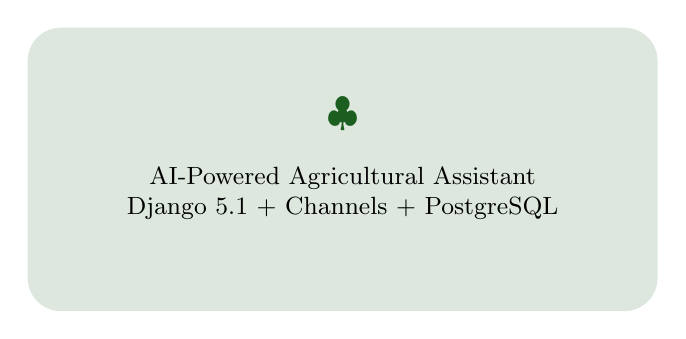
\begin{tikzpicture}
    \fill[primary!15, rounded corners=12pt] (-4,-1.8) rectangle (4,1.8);
    \node[font=\Large] at (0,0.7) {\textcolor{primary}{$\clubsuit$}};
    \node[font=\small, text width=6cm, align=center] at (0,-0.3)
        {AI-Powered Agricultural Assistant\\Django 5.1 + Channels + PostgreSQL};
\end{tikzpicture}

\vspace{2cm}

\begin{tabular}{ll}
    \textbf{Version} & 1.0 \\
    \textbf{Date} & February 2026 \\
    \textbf{Framework} & Django 5.1 (ASGI) \\
    \textbf{Database} & PostgreSQL 16 \\
    \textbf{Auth} & JWT (HS256) via SimpleJWT \\
\end{tabular}

\vfill
{\small KhetiMitra Engineering Team}
\end{titlepage}

% ── Table of Contents ─────────────────────────────────────────────────
\tableofcontents
\newpage

% ══════════════════════════════════════════════════════════════════════
\section{Architecture Overview}
% ══════════════════════════════════════════════════════════════════════

\subsection{System Architecture Diagram}

\begin{figure}[H]
\centering
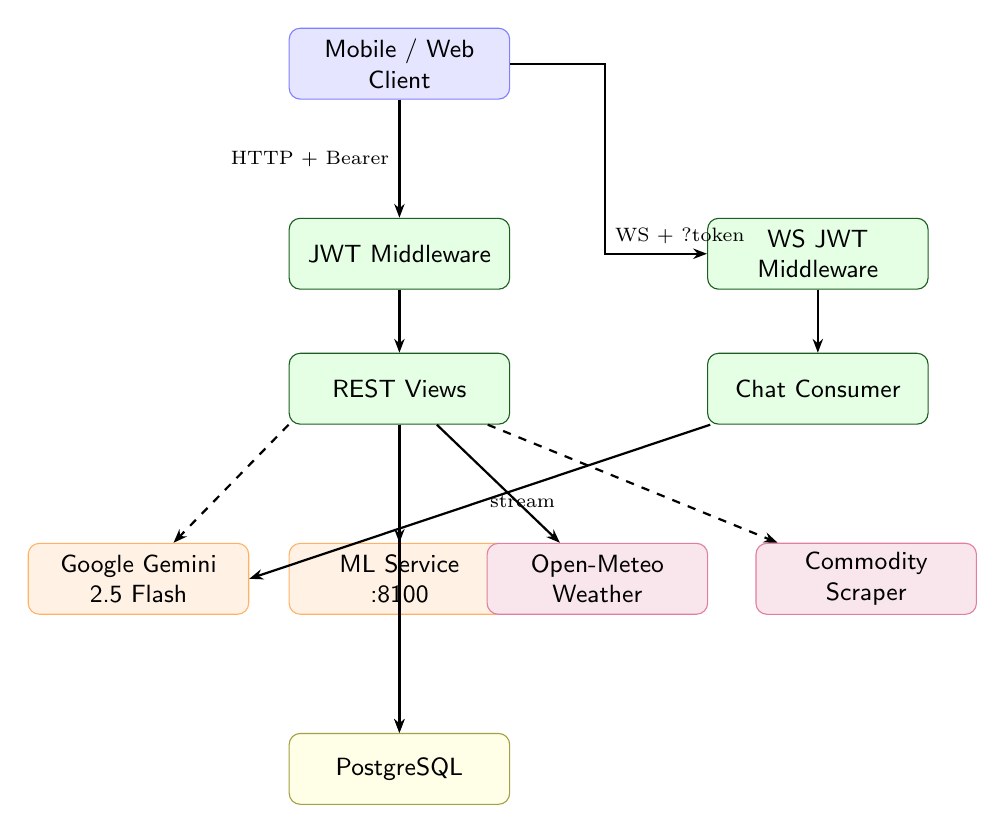
\begin{tikzpicture}[
    node distance=1.2cm and 1.8cm,
    every node/.style={font=\small},
    box/.style={rectangle, draw, rounded corners=4pt, minimum width=2.8cm,
                minimum height=0.9cm, align=center, font=\small\sffamily},
    clientbox/.style={box, fill=blue!10, draw=blue!50},
    djangobox/.style={box, fill=green!10, draw=primary},
    aibox/.style={box, fill=orange!10, draw=orange!60},
    extbox/.style={box, fill=purple!10, draw=purple!50},
    dbbox/.style={box, fill=yellow!10, draw=yellow!60!black},
    arr/.style={-{Stealth[length=5pt]}, thick},
    darr/.style={-{Stealth[length=5pt]}, thick, dashed},
]
    % Client
    \node[clientbox] (app) {Mobile / Web\\Client};

    % Django layer
    \node[djangobox, below=1.5cm of app] (mw) {JWT Middleware};
    \node[djangobox, below=0.8cm of mw] (views) {REST Views};
    \node[djangobox, right=2.5cm of mw] (wsmw) {WS JWT\\Middleware};
    \node[djangobox, below=0.8cm of wsmw] (consumer) {Chat Consumer};

    % AI & External
    \node[aibox, below left=1.5cm and 0.5cm of views] (gemini) {Google Gemini\\2.5 Flash};
    \node[aibox, below=1.5cm of views] (ml) {ML Service\\:8100};
    \node[extbox, below right=1.5cm and -0.3cm of views] (weather) {Open-Meteo\\Weather};
    \node[extbox, right=0.6cm of weather] (mandi) {Commodity\\Scraper};

    % Database
    \node[dbbox, below=1.5cm of ml] (db) {PostgreSQL};

    % Arrows
    \draw[arr] (app) -- node[left, font=\scriptsize]{HTTP + Bearer} (mw);
    \draw[arr] (mw) -- (views);
    \draw[arr] (app.east) -- ++(1.2,0) |- node[above right, font=\scriptsize]{WS + ?token} (wsmw);
    \draw[arr] (wsmw) -- (consumer);
    \draw[arr] (consumer) -- node[right, font=\scriptsize]{stream} (gemini.east);
    \draw[arr] (views) -- (ml);
    \draw[arr] (views) -- (weather);
    \draw[darr] (views) -- (mandi);
    \draw[arr] (views) -- (db);
    \draw[arr] (ml) -- (db);
    \draw[darr] (views.south west) -- (gemini);
    
\end{tikzpicture}
\caption{KhetiMitra System Architecture}
\end{figure}

\subsection{Component Map}

\begin{table}[H]
\centering
\begin{tabularx}{\textwidth}{l l X}
\toprule
\textbf{Layer} & \textbf{File} & \textbf{Responsibility} \\
\midrule
Entry Point    & \texttt{asgi.py}        & ASGI application, routes HTTP and WebSocket \\
HTTP Routing   & \texttt{urls.py}        & Maps URL paths to view functions \\
WS Routing     & \texttt{routing.py}     & Maps WebSocket paths to consumers \\
Auth (HTTP)    & \texttt{middleware.py}   & Validates Bearer JWT on all \texttt{/api/*} paths \\
Auth (WS)      & \texttt{wsmiddleware.py} & Validates JWT from query string on WS connect \\
Views          & \texttt{views.py}       & All REST endpoint handlers \\
Consumer       & \texttt{consumer.py}    & Real-time AI chat via WebSocket \\
Models         & \texttt{models.py}      & Django ORM -- Farmer, Land, Plan \\
Utilities      & \texttt{utilities.py}   & Weather API, Gemini AI helpers \\
Price API      & \texttt{price\_api.py}  & Selenium-based mandi price scraper \\
Chat Model     & \texttt{chatmodel.py}   & Gemini 2.5 Flash streaming client \\
Settings       & \texttt{settings.py}    & Django config, JWT, DB, middleware \\
\bottomrule
\end{tabularx}
\caption{File-to-Responsibility Map}
\end{table}

\subsection{Tech Stack}

\begin{table}[H]
\centering
\begin{tabular}{l l}
\toprule
\textbf{Category} & \textbf{Technology} \\
\midrule
Framework       & Django 5.1 + Django REST Framework \\
Async/WebSocket & Django Channels (InMemoryChannelLayer) \\
Database        & PostgreSQL 16 \\
Authentication  & \texttt{djangorestframework-simplejwt} (HS256) \\
AI Engine       & Google Gemini 2.5 Flash (streaming) \\
Weather Data    & Open-Meteo API (cached 1h) \\
Market Data     & Selenium headless Chrome scraper \\
ML Microservice & External service at \texttt{localhost:8100} \\
Server          & ASGI (Daphne / Uvicorn) \\
\bottomrule
\end{tabular}
\end{table}

% ══════════════════════════════════════════════════════════════════════
\newpage
\section{Database Schema}
% ══════════════════════════════════════════════════════════════════════

\subsection{Entity Relationship Diagram}

\begin{figure}[H]
\centering
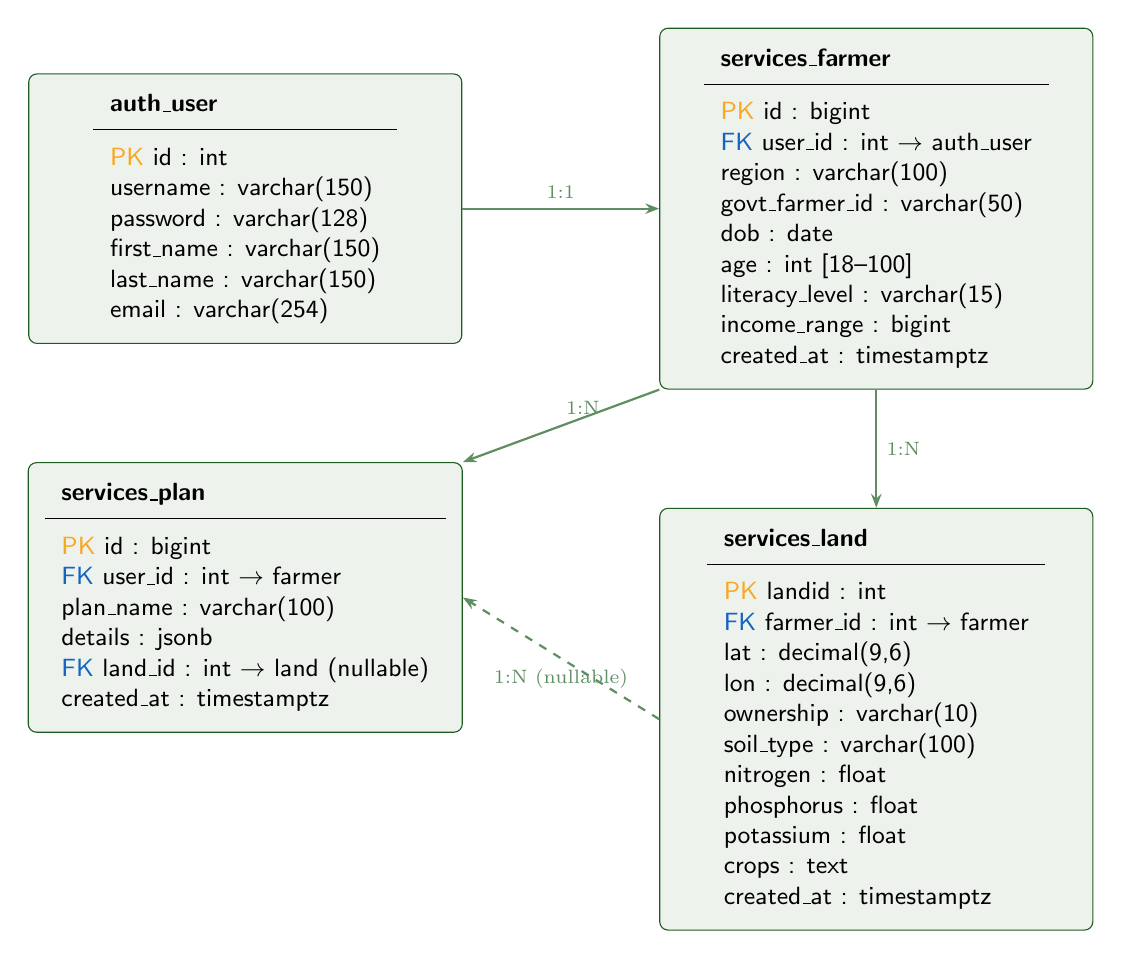
\begin{tikzpicture}[
    node distance=0.5cm,
    entity/.style={rectangle, draw=primary, fill=primary!8, rounded corners=3pt,
                   minimum width=5.5cm, font=\small\sffamily, inner sep=6pt},
    attr/.style={font=\scriptsize\ttfamily, text=black!80},
    rel/.style={-{Stealth[length=5pt]}, thick, primary!70},
]
    % auth_user
    \node[entity] (user) {
        \begin{tabular}{l}
            \textbf{auth\_user} \\[3pt]
            \hline \\[-6pt]
            \textcolor{lockgold}{PK} id : int \\
            username : varchar(150) \\
            password : varchar(128) \\
            first\_name : varchar(150) \\
            last\_name : varchar(150) \\
            email : varchar(254) \\
        \end{tabular}
    };

    % Farmer
    \node[entity, right=2.5cm of user] (farmer) {
        \begin{tabular}{l}
            \textbf{services\_farmer} \\[3pt]
            \hline \\[-6pt]
            \textcolor{lockgold}{PK} id : bigint \\
            \textcolor{urlblue}{FK} user\_id : int $\to$ auth\_user \\
            region : varchar(100) \\
            govt\_farmer\_id : varchar(50) \\
            dob : date \\
            age : int [18--100] \\
            literacy\_level : varchar(15) \\
            income\_range : bigint \\
            created\_at : timestamptz \\
        \end{tabular}
    };

    % Land
    \node[entity, below=1.5cm of farmer] (land) {
        \begin{tabular}{l}
            \textbf{services\_land} \\[3pt]
            \hline \\[-6pt]
            \textcolor{lockgold}{PK} landid : int \\
            \textcolor{urlblue}{FK} farmer\_id : int $\to$ farmer \\
            lat : decimal(9,6) \\
            lon : decimal(9,6) \\
            ownership : varchar(10) \\
            soil\_type : varchar(100) \\
            nitrogen : float \\
            phosphorus : float \\
            potassium : float \\
            crops : text \\
            created\_at : timestamptz \\
        \end{tabular}
    };

    % Plan
    \node[entity, below=1.5cm of user] (plan) {
        \begin{tabular}{l}
            \textbf{services\_plan} \\[3pt]
            \hline \\[-6pt]
            \textcolor{lockgold}{PK} id : bigint \\
            \textcolor{urlblue}{FK} user\_id : int $\to$ farmer \\
            plan\_name : varchar(100) \\
            details : jsonb \\
            \textcolor{urlblue}{FK} land\_id : int $\to$ land (nullable) \\
            created\_at : timestamptz \\
        \end{tabular}
    };

    % Relationships
    \draw[rel] (user.east) -- node[above, font=\scriptsize]{1:1} (farmer.west);
    \draw[rel] (farmer.south) -- node[right, font=\scriptsize]{1:N} (land.north);
    \draw[rel] (farmer.south west) -- node[left, font=\scriptsize, near start]{1:N} (plan.north east);
    \draw[rel, dashed] (land.west) -- node[below, font=\scriptsize]{1:N (nullable)} (plan.east);

\end{tikzpicture}
\caption{Entity Relationship Diagram}
\end{figure}

\subsection{Table: \texttt{auth\_user} (Django Built-in)}

Django's default User model. The \texttt{username} field stores \texttt{"FAR" + phone\_number} as a unique identifier (e.g., \texttt{FAR9876543210}).

\begin{table}[H]
\centering
\begin{tabularx}{\textwidth}{l l l X}
\toprule
\textbf{Column} & \textbf{Type} & \textbf{Constraint} & \textbf{Notes} \\
\midrule
\texttt{id}         & \texttt{int}          & PK, auto    & \\
\texttt{username}   & \texttt{varchar(150)} & Unique      & Stores \texttt{FAR\{phone\}} \\
\texttt{password}   & \texttt{varchar(128)} &             & PBKDF2 hashed \\
\texttt{first\_name} & \texttt{varchar(150)} &             & \\
\texttt{last\_name}  & \texttt{varchar(150)} &             & \\
\texttt{email}      & \texttt{varchar(254)} &             & \\
\bottomrule
\end{tabularx}
\end{table}

\subsection{Table: \texttt{services\_farmer}}

\begin{table}[H]
\centering
\begin{tabularx}{\textwidth}{l l l X}
\toprule
\textbf{Column} & \textbf{Type} & \textbf{Constraint} & \textbf{Notes} \\
\midrule
\texttt{id}              & \texttt{bigint}       & PK, auto             & \\
\texttt{user\_id}        & \texttt{int}          & FK $\to$ auth\_user, Unique & OneToOne \\
\texttt{region}          & \texttt{varchar(100)} & Nullable             & e.g.\ ``Maharashtra'' \\
\texttt{govt\_farmer\_id} & \texttt{varchar(50)}  & Nullable             & Government ID \\
\texttt{dob}             & \texttt{date}         & Nullable             & Date of birth \\
\texttt{age}             & \texttt{int}          & 18 $\leq$ x $\leq$ 100 & Auto-calc from dob \\
\texttt{literacy\_level} & \texttt{varchar(15)}  & Required             & ILLITERATE, BASIC, FLUENT \\
\texttt{income\_range}   & \texttt{bigint}       & Nullable             & Annual income \\
\texttt{created\_at}     & \texttt{timestamptz}  & Auto                 & \\
\bottomrule
\end{tabularx}
\end{table}

\subsection{Table: \texttt{services\_land}}

\begin{table}[H]
\centering
\begin{tabularx}{\textwidth}{l l l X}
\toprule
\textbf{Column} & \textbf{Type} & \textbf{Constraint} & \textbf{Notes} \\
\midrule
\texttt{landid}     & \texttt{int}           & PK          & Auto-generated composite key \\
\texttt{farmer\_id} & \texttt{int}           & FK $\to$ farmer & CASCADE \\
\texttt{lat}        & \texttt{decimal(9,6)}  & Nullable    & GPS latitude \\
\texttt{lon}        & \texttt{decimal(9,6)}  & Nullable    & GPS longitude \\
\texttt{ownership}  & \texttt{varchar(10)}   & Required    & OWNER $|$ RENTED \\
\texttt{soil\_type} & \texttt{varchar(100)}  & Required    & From image analysis \\
\texttt{nitrogen}   & \texttt{float}         & Min 0.1     & From image analysis \\
\texttt{phosphorus} & \texttt{float}         & Nullable    & From image analysis \\
\texttt{potassium}  & \texttt{float}         & Nullable    & From image analysis \\
\texttt{crops}      & \texttt{text}          & Nullable    & Past/eligible crops \\
\texttt{created\_at} & \texttt{timestamptz}  & Auto        & \\
\bottomrule
\end{tabularx}
\end{table}

\subsection{Table: \texttt{services\_plan}}

\begin{table}[H]
\centering
\begin{tabularx}{\textwidth}{l l l X}
\toprule
\textbf{Column} & \textbf{Type} & \textbf{Constraint} & \textbf{Notes} \\
\midrule
\texttt{id}          & \texttt{bigint}       & PK, auto    & \\
\texttt{user\_id}    & \texttt{int}          & FK $\to$ farmer & CASCADE \\
\texttt{plan\_name}  & \texttt{varchar(100)} & Auto-gen    & \texttt{\{name\}PLAN\{uuid8\}\{ts\}} \\
\texttt{details}     & \texttt{jsonb}        & Required    & AI-generated farming plan \\
\texttt{land\_id}    & \texttt{int}          & FK $\to$ land, Nullable & Associated land parcel \\
\texttt{created\_at} & \texttt{timestamptz}  & Auto        & \\
\bottomrule
\end{tabularx}
\end{table}

% ══════════════════════════════════════════════════════════════════════
\newpage
\section{JWT Authentication \& Flow}
% ══════════════════════════════════════════════════════════════════════

\subsection{JWT Configuration}

\begin{lstlisting}[style=jsonStyle, title={\texttt{settings.py} -- SIMPLE\_JWT}]
SIMPLE_JWT = {
    'ACCESS_TOKEN_LIFETIME': timedelta(days=1),   # 24 hours
    'REFRESH_TOKEN_LIFETIME': timedelta(days=7),  # 7 days
    'ROTATE_REFRESH_TOKENS': False,
    'ALGORITHM': 'HS256',
    'SIGNING_KEY': SECRET_KEY,
    'AUTH_HEADER_TYPES': ('Bearer',),
}
\end{lstlisting}

\subsection{Token Structure (HS256)}

\begin{lstlisting}[style=jsonStyle, title={JWT Payload (decoded)}]
Header:  { "alg": "HS256", "typ": "JWT" }

Payload: {
    "token_type": "access",
    "exp": 1707696000,
    "iat": 1707609600,
    "jti": "a1b2c3d4...",
    "user_id": 5
}

Signature: HMACSHA256(base64(header) + "." + base64(payload), SECRET_KEY)
\end{lstlisting}

\subsection{Authentication Flow Diagram}

\begin{figure}[H]
\centering
\begin{tikzpicture}[
    node distance=0.6cm,
    step/.style={rectangle, draw=primary!60, fill=primary!5, rounded corners=3pt,
                 minimum width=11cm, minimum height=0.7cm, font=\small, align=left, inner sep=6pt},
    label/.style={font=\small\bfseries\color{primary}},
    arr/.style={-{Stealth[length=4pt]}, thick, primary!50},
]
    % Login Flow
    \node[label] (l1) {Login Flow (Token Generation)};
    \node[step, below=0.3cm of l1]  (s1) {1. Client sends \texttt{POST /api/login/} with \texttt{phone\_number} + \texttt{password}};
    \node[step, below=0.15cm of s1] (s2) {2. View authenticates: \texttt{authenticate(username="FAR"+phone, password)}};
    \node[step, below=0.15cm of s2] (s3) {3. On success: \texttt{RefreshToken.for\_user(user)} generates access + refresh tokens};
    \node[step, below=0.15cm of s3] (s4) {4. Returns JSON: \texttt{\{access\_token, refresh\_token, user\_details\}}};

    \draw[arr] (s1.south west) -- (s2.north west);
    \draw[arr] (s2.south west) -- (s3.north west);
    \draw[arr] (s3.south west) -- (s4.north west);

    % Validation Flow
    \node[label, below=0.8cm of s4] (l2) {Protected Request (Token Validation via Middleware)};
    \node[step, below=0.3cm of l2]  (v1) {1. Client sends request with header: \texttt{Authorization: Bearer eyJ...}};
    \node[step, below=0.15cm of v1] (v2) {2. \texttt{JWTManualValidator} checks path -- skip if \texttt{/api/signup/} or \texttt{/api/login/}};
    \node[step, below=0.15cm of v2] (v3) {3. Extracts token, calls \texttt{JWTAuthentication().get\_validated\_token(token)}};
    \node[step, below=0.15cm of v3] (v4) {4. SimpleJWT decodes HS256, verifies signature, checks expiry};
    \node[step, below=0.15cm of v4] (v5) {5. \texttt{get\_user(validated\_token)} retrieves User from DB, sets \texttt{request.user}};
    \node[step, below=0.15cm of v5] (v6) {6. Request passes through to the view function};

    \draw[arr] (v1.south west) -- (v2.north west);
    \draw[arr] (v2.south west) -- (v3.north west);
    \draw[arr] (v3.south west) -- (v4.north west);
    \draw[arr] (v4.south west) -- (v5.north west);
    \draw[arr] (v5.south west) -- (v6.north west);

\end{tikzpicture}
\caption{JWT Authentication Flow}
\end{figure}

\subsection{Middleware Pipeline}

The \texttt{JWTManualValidator} runs \textbf{first} in the middleware stack:

\begin{center}
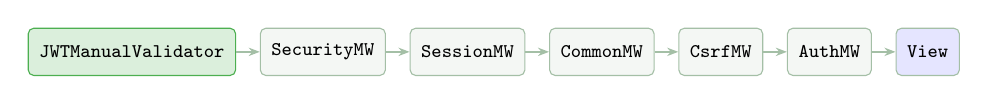
\begin{tikzpicture}[
    mw/.style={rectangle, draw=primary!40, fill=primary!5, rounded corners=2pt,
               minimum height=0.6cm, font=\scriptsize\ttfamily, inner sep=4pt},
    arr/.style={-{Stealth[length=4pt]}, thick, primary!40},
]
    \node[mw, fill=accent!20, draw=accent] (j) {JWTManualValidator};
    \node[mw, right=0.3cm of j] (sec) {SecurityMW};
    \node[mw, right=0.3cm of sec] (ses) {SessionMW};
    \node[mw, right=0.3cm of ses] (com) {CommonMW};
    \node[mw, right=0.3cm of com] (csrf) {CsrfMW};
    \node[mw, right=0.3cm of csrf] (auth) {AuthMW};
    \node[mw, right=0.3cm of auth, fill=blue!10] (view) {View};

    \draw[arr] (j) -- (sec);
    \draw[arr] (sec) -- (ses);
    \draw[arr] (ses) -- (com);
    \draw[arr] (com) -- (csrf);
    \draw[arr] (csrf) -- (auth);
    \draw[arr] (auth) -- (view);
\end{tikzpicture}
\end{center}

\subsection{Auth-Required Matrix}

\begin{table}[H]
\centering
\begin{tabular}{l l c l}
\toprule
\textbf{Endpoint} & \textbf{Method} & \textbf{Auth?} & \textbf{Middleware} \\
\midrule
\texttt{/api/signup/}      & POST & \publicbadge  & -- \\
\texttt{/api/login/}       & POST & \publicbadge  & -- \\
\texttt{/api/weather/}     & GET  & \authbadge    & JWTManualValidator \\
\texttt{/api/market/}      & GET  & \authbadge    & JWTManualValidator \\
\texttt{/api/plans/}       & GET  & \authbadge    & JWTManualValidator \\
\texttt{/api/plans/add/}   & POST & \authbadge    & JWTManualValidator \\
\texttt{/api/recommend/}   & GET  & \authbadge    & JWTManualValidator \\
\texttt{/api/diagnosis/}   & POST & \authbadge    & JWTManualValidator \\
\texttt{/api/lands/}       & GET  & \authbadge    & JWTManualValidator \\
\texttt{/api/lands/add/}   & POST & \authbadge    & JWTManualValidator \\
\texttt{/ws/chat/}         & WS   & \authbadge    & JWTAuthMiddleware (query) \\
\bottomrule
\end{tabular}
\caption{Authentication Requirements per Endpoint}
\end{table}

\subsection{WebSocket Authentication}

WebSocket connections pass the JWT as a query parameter:

\begin{lstlisting}[style=bashStyle]
ws://localhost:8000/ws/chat/?token=eyJhbGciOiJIUzI1NiIs...
\end{lstlisting}

The \texttt{JWTAuthMiddleware} (in \texttt{wsmiddleware.py}):
\begin{enumerate}[noitemsep]
    \item Extracts \texttt{token} from the query string
    \item Validates it using \texttt{AccessToken(token\_key)}
    \item Retrieves User via \texttt{user\_id} claim
    \item Attaches user to \texttt{scope["user"]}
\end{enumerate}

% ══════════════════════════════════════════════════════════════════════
\newpage
\section{API Reference}
% ══════════════════════════════════════════════════════════════════════

\begin{infobox}
\textbf{Base URL:} \texttt{http://localhost:8000/} \\
\textbf{WebSocket:} \texttt{ws://localhost:8000/ws/chat/} \\
\textbf{Content-Type (forms):} \texttt{application/x-www-form-urlencoded} \\
\textbf{Content-Type (JSON):} \texttt{application/json}
\end{infobox}

% ── 1. Signup ─────────────────────────────────────────────────────────
\subsection{\httpmethod{POST} \texttt{/api/signup/} \hfill \publicbadge}

Register a new farmer. Creates both a Django \texttt{User} and a linked \texttt{Farmer} profile atomically.

\subsubsection*{Request Body (\texttt{form-urlencoded})}

\begin{table}[H]
\centering
\begin{tabularx}{\textwidth}{l l c X}
\toprule
\textbf{Field} & \textbf{Type} & \textbf{Req} & \textbf{Description} \\
\midrule
\texttt{phone\_number}    & string  & \checkmark & e.g.\ \texttt{9876543210} \\
\texttt{password}         & string  & \checkmark & Min 8 chars (Django validators) \\
\texttt{first\_name}      & string  &            & \\
\texttt{last\_name}       & string  &            & \\
\texttt{email}            & string  &            & \\
\texttt{region}           & string  &            & e.g.\ ``Maharashtra'' \\
\texttt{govt\_farmer\_id} & string  &            & Government-issued ID \\
\texttt{dob}              & string  & \checkmark & Format: \texttt{YYYY-MM-DD} \\
\texttt{literacy\_level}  & string  &            & \texttt{ILLITERATE}, \texttt{BASIC} (default), \texttt{FLUENT} \\
\texttt{income\_range}    & integer &            & Annual income \\
\bottomrule
\end{tabularx}
\end{table}

\subsubsection*{Response -- \texttt{201 Created}}
\begin{lstlisting}[style=jsonStyle]
{
    "status": "success",
    "username": "FAR9876543210",
    "message": "User and Profile created successfully"
}
\end{lstlisting}

\subsubsection*{Error -- \texttt{400 Bad Request}}
\begin{lstlisting}[style=jsonStyle]
{ "error": "UNIQUE constraint failed: auth_user.username", "type": "inbound" }
\end{lstlisting}

% ── 2. Login ──────────────────────────────────────────────────────────
\subsection{\httpmethod{POST} \texttt{/api/login/} \hfill \publicbadge}

Authenticate with phone number and password. Returns JWT access and refresh tokens.

\subsubsection*{Request Body (\texttt{form-urlencoded})}

\begin{table}[H]
\centering
\begin{tabularx}{\textwidth}{l l c X}
\toprule
\textbf{Field} & \textbf{Type} & \textbf{Req} & \textbf{Description} \\
\midrule
\texttt{phone\_number} & string & \checkmark & Raw phone number \\
\texttt{password}       & string & \checkmark & \\
\bottomrule
\end{tabularx}
\end{table}

\subsubsection*{Response -- \texttt{200 OK}}
\begin{lstlisting}[style=jsonStyle]
{
    "access_token": "eyJhbGciOiJIUzI1NiIs...",
    "refresh_token": "eyJhbGciOiJIUzI1NiIs...",
    "user_details": {
        "first_name": "Ravi",
        "last_name": "Kumar",
        "phone": "9876543210"
    }
}
\end{lstlisting}

\subsubsection*{Error -- \texttt{401 Unauthorized}}
\begin{lstlisting}[style=jsonStyle]
{ "error": "Invalid phone or password" }
\end{lstlisting}

% ── 3. Weather ────────────────────────────────────────────────────────
\subsection{\httpmethod{GET} \texttt{/api/weather/} \hfill \authbadge}

Fetch 16-day weather forecast from Open-Meteo API (cached 1 hour).

\subsubsection*{Query Parameters}

\begin{table}[H]
\centering
\begin{tabular}{l l c l l}
\toprule
\textbf{Param} & \textbf{Type} & \textbf{Req} & \textbf{Default} & \textbf{Description} \\
\midrule
\texttt{lat} & float & & 20 & Latitude \\
\texttt{lon} & float & & 10 & Longitude \\
\bottomrule
\end{tabular}
\end{table}

\subsubsection*{Response -- \texttt{200 OK}}
\begin{lstlisting}[style=jsonStyle]
{
    "metadata": { "lat": 19.0, "lon": 72.8, "elevation": 14.0, "timezone": "Asia/Kolkata" },
    "current": {
        "time": 1707609600, "temp": 28.5, "humidity": 65.0,
        "precipitation": 0.0, "is_day": true, "feels_like": 30.2
    },
    "daily": [
        { "date": "2026-02-10", "weather_code": 1, "temp_max": 32.5,
          "temp_min": 22.1, "rain_sum_mm": 0.0, "precip_prob": 10.0 }
    ]
}
\end{lstlisting}

% ── 4. Market ─────────────────────────────────────────────────────────
\subsection{\httpmethod{GET} \texttt{/api/market/} \hfill \authbadge}

Fetch mandi commodity prices via Selenium scraper (CommodityOnline).

\subsubsection*{Query Parameters}

\begin{table}[H]
\centering
\begin{tabular}{l l c l l}
\toprule
\textbf{Param} & \textbf{Type} & \textbf{Req} & \textbf{Default} & \textbf{Description} \\
\midrule
\texttt{state} & string & & Mumbai  & State name \\
\texttt{mandi} & string & & ok      & Mandi name \\
\texttt{crop}  & string & & wheat   & Crop name \\
\bottomrule
\end{tabular}
\end{table}

\subsubsection*{Response -- \texttt{200 OK}}
\begin{lstlisting}[style=jsonStyle]
{
    "meta": { "Commodity": "Wheat", "State": "Maharashtra", "District": "Ahmednagar" },
    "prices": { "27/12/2025": 2650.0, "26/12/2025": 2600.0 }
}
\end{lstlisting}

% ── 5. Plans ──────────────────────────────────────────────────────────
\subsection{\httpmethod{GET} \texttt{/api/plans/} \hfill \authbadge}

Get all plans for the authenticated farmer. Optionally filter by plan ID.

\subsubsection*{Query Parameters}

\begin{table}[H]
\centering
\begin{tabular}{l l c l}
\toprule
\textbf{Param} & \textbf{Type} & \textbf{Req} & \textbf{Description} \\
\midrule
\texttt{id} & int & & Specific plan ID \\
\bottomrule
\end{tabular}
\end{table}

\subsubsection*{Response -- \texttt{200 OK} (all plans)}
\begin{lstlisting}[style=jsonStyle]
[
    {
        "id": 1, "user_id": 3,
        "plan_name": "RaviPLAN12345671707609600",
        "details": { "...AI-generated plan..." },
        "land_id": 1, "created_at": "2026-02-10T07:30:00Z"
    }
]
\end{lstlisting}

% ── 6. Add Plan ───────────────────────────────────────────────────────
\subsection{\httpmethod{POST} \texttt{/api/plans/add/} \hfill \authbadge}

Generate an AI farming plan for a specific crop and land parcel.

\subsubsection*{Request Body (JSON)}
\begin{lstlisting}[style=jsonStyle]
{ "crop": "rice", "land_id": 1 }
\end{lstlisting}

\subsubsection*{Response -- \texttt{200 OK}}
\begin{lstlisting}[style=jsonStyle]
{ "message": "Plan added", "id": 5, "plan": { "...AI-generated farming plan..." } }
\end{lstlisting}

% ── 7. Crop Recommendation ───────────────────────────────────────────
\subsection{\httpmethod{GET} \texttt{/api/recommend/} \hfill \authbadge}

AI-powered crop recommendation using land soil data + live weather.

\subsubsection*{Query Parameters}

\begin{table}[H]
\centering
\begin{tabular}{l l c l l}
\toprule
\textbf{Param} & \textbf{Type} & \textbf{Req} & \textbf{Default} & \textbf{Description} \\
\midrule
\texttt{land\_id} & int & & 80 & Land parcel ID \\
\bottomrule
\end{tabular}
\end{table}

\subsubsection*{Internal Flow}
\begin{enumerate}[noitemsep]
    \item Fetches Land record (N, P, K, lat, lon, ph) from DB
    \item Fetches live weather (humidity, rainfall, temperature) from Open-Meteo
    \item POSTs combined data to ML service at \texttt{localhost:8100/recommend/}
    \item Returns ML prediction
\end{enumerate}

\subsubsection*{Response -- \texttt{200 OK}}
\begin{lstlisting}[style=jsonStyle]
{ "recommended_crop": "rice", "confidence": 0.92, "alternatives": ["wheat", "maize"] }
\end{lstlisting}

% ── 8. Plant Diagnosis ───────────────────────────────────────────────
\subsection{\httpmethod{POST} \texttt{/api/diagnosis/} \hfill \authbadge}

Upload a plant photo for disease diagnosis. Uses ML + Google Gemini for detailed report.

\subsubsection*{Request Body (\texttt{multipart/form-data})}

\begin{table}[H]
\centering
\begin{tabularx}{\textwidth}{l l c X}
\toprule
\textbf{Field} & \textbf{Type} & \textbf{Req} & \textbf{Description} \\
\midrule
\texttt{image} & file & \checkmark & Photo of plant leaf/stem \\
\bottomrule
\end{tabularx}
\end{table}

\subsubsection*{Internal Flow}
\begin{enumerate}[noitemsep]
    \item Saves uploaded image to \texttt{media/lands/}
    \item Sends file path to ML service \texttt{localhost:8100/plant/}
    \item Passes ML result to Google Gemini for a detailed AI report
    \item Returns diagnosis text
\end{enumerate}

\subsubsection*{Response -- \texttt{200 OK}}
\begin{lstlisting}[style=jsonStyle]
{ "diagnosis": "The plant appears to have bacterial leaf blight. Treatment: ..." }
\end{lstlisting}

% ── 9. Get Lands ─────────────────────────────────────────────────────
\subsection{\httpmethod{GET} \texttt{/api/lands/} \hfill \authbadge}

Get all land parcels for the authenticated farmer.

\subsubsection*{Response -- \texttt{200 OK}}
\begin{lstlisting}[style=jsonStyle]
[
    {
        "landid": 123456, "farmer_id": 3,
        "lat": "19.076090", "lon": "72.877426",
        "ownership": "OWNER", "soil_type": "Red Loamy",
        "nitrogen": 45.2, "phosphorus": 12.5, "potassium": 30.0,
        "crops": "rice, wheat", "created_at": "2026-01-15T10:30:00Z"
    }
]
\end{lstlisting}

% ── 10. Add Land ─────────────────────────────────────────────────────
\subsection{\httpmethod{POST} \texttt{/api/lands/add/} \hfill \authbadge}

Register a new land parcel with soil image analysis.

\subsubsection*{Request Body (\texttt{multipart/form-data})}

\begin{table}[H]
\centering
\begin{tabularx}{\textwidth}{l l c X}
\toprule
\textbf{Field} & \textbf{Type} & \textbf{Req} & \textbf{Description} \\
\midrule
\texttt{image}     & file    & \checkmark & Soil photograph \\
\texttt{lat}       & decimal &            & GPS latitude \\
\texttt{lon}       & decimal &            & GPS longitude \\
\texttt{ownership} & string  &            & \texttt{OWNER} (default) or \texttt{RENTED} \\
\bottomrule
\end{tabularx}
\end{table}

\subsubsection*{Internal Flow}
\begin{enumerate}[noitemsep]
    \item Saves soil image to \texttt{media/lands/}
    \item Sends to ML service \texttt{localhost:8100/soil/} for analysis
    \item Creates \texttt{Land} record with extracted: soil\_type, N, P, K, ph, organic\_matter, eligible\_crops
\end{enumerate}

\subsubsection*{Response -- \texttt{200 OK}}
\begin{lstlisting}[style=jsonStyle]
{
    "message": "Land added", "id": 123456,
    "analysis": {
        "soil_type": "Red Loamy", "nitrogen": 45.2,
        "phosphorus": 12.5, "potassium": 30.0,
        "ph": 6.5, "organic_matter": "Medium",
        "eligible_crops": "rice, wheat, soybean"
    }
}
\end{lstlisting}

% ══════════════════════════════════════════════════════════════════════
\newpage
\section{WebSocket API}
% ══════════════════════════════════════════════════════════════════════

\subsection{Endpoint}

\begin{lstlisting}[style=bashStyle]
ws://localhost:8000/ws/chat/?token=<JWT_ACCESS_TOKEN>
\end{lstlisting}

\subsection{Connection Flow Diagram}

\begin{figure}[H]
\centering
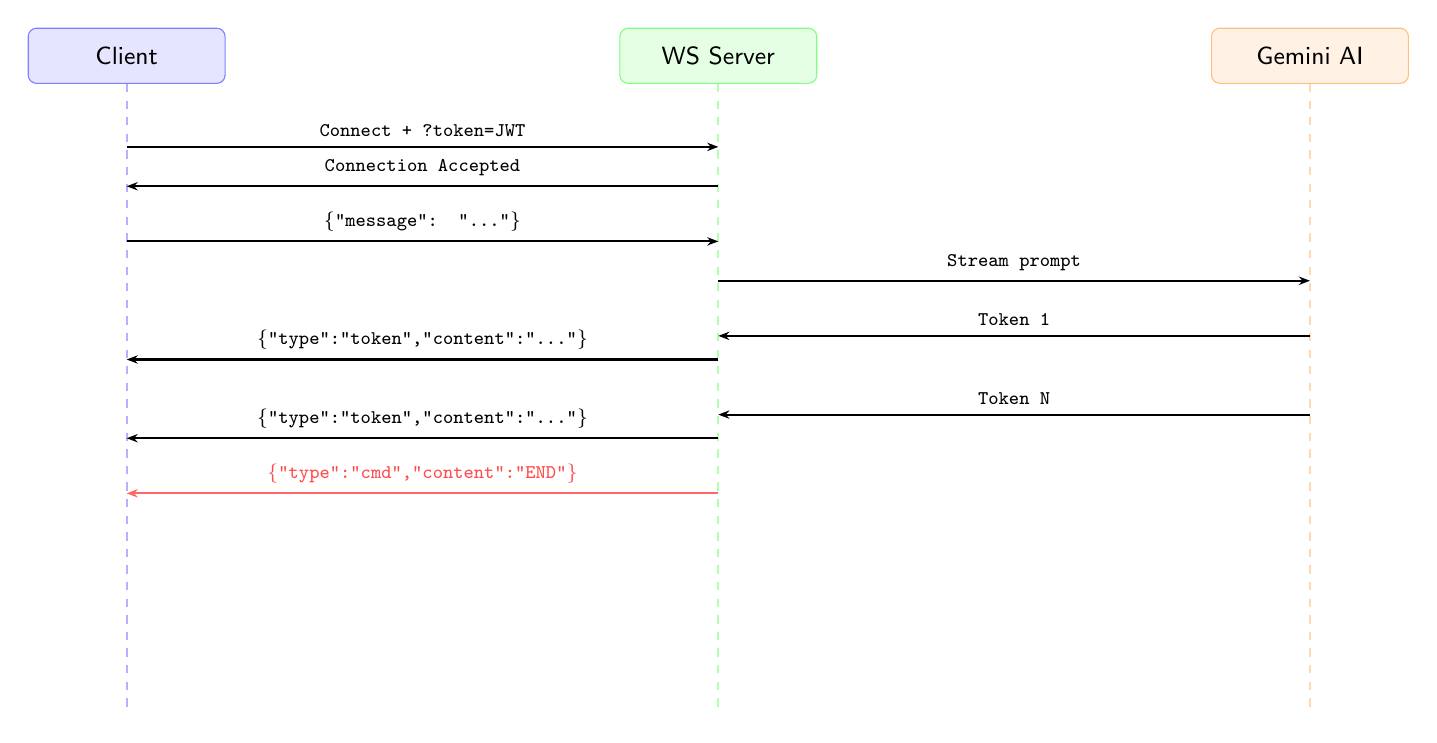
\begin{tikzpicture}[
    node distance=0.4cm,
    actor/.style={rectangle, draw, rounded corners=3pt, minimum width=2.5cm,
                  minimum height=0.7cm, font=\small\sffamily, fill=#1!10, draw=#1!50},
    msg/.style={font=\scriptsize\ttfamily},
    arr/.style={-{Stealth[length=4pt]}, thick},
]
    % Actors
    \node[actor=blue] (client) {Client};
    \node[actor=green, right=5cm of client] (server) {WS Server};
    \node[actor=orange, right=5cm of server] (ai) {Gemini AI};

    % Lifelines
    \draw[thick, dashed, blue!30] (client.south) -- ++(0,-8);
    \draw[thick, dashed, green!30] (server.south) -- ++(0,-8);
    \draw[thick, dashed, orange!30] (ai.south) -- ++(0,-8);

    % Messages
    \coordinate (c) at ($(client.south)+(0,-0.8)$);
    \coordinate (s) at ($(server.south)+(0,-0.8)$);
    \coordinate (a) at ($(ai.south)+(0,-0.8)$);

    \draw[arr] (c) -- node[above, msg]{Connect + ?token=JWT} (s);
    \draw[arr] ($(s)+(0,-0.5)$) -- node[above, msg]{Connection Accepted} ($(c)+(0,-0.5)$);
    
    \draw[arr] ($(c)+(0,-1.2)$) -- node[above, msg]{\{"message": "..."\}} ($(s)+(0,-1.2)$);
    \draw[arr] ($(s)+(0,-1.7)$) -- node[above, msg]{Stream prompt} ($(a)+(0,-1.7)$);
    
    \draw[arr] ($(a)+(0,-2.4)$) -- node[above, msg]{Token 1} ($(s)+(0,-2.4)$);
    \draw[arr] ($(s)+(0,-2.7)$) -- node[above, msg]{\{"type":"token","content":"..."\}} ($(c)+(0,-2.7)$);
    
    \draw[arr] ($(a)+(0,-3.4)$) -- node[above, msg]{Token N} ($(s)+(0,-3.4)$);
    \draw[arr] ($(s)+(0,-3.7)$) -- node[above, msg]{\{"type":"token","content":"..."\}} ($(c)+(0,-3.7)$);
    
    \draw[arr, red!60] ($(s)+(0,-4.4)$) -- node[above, msg, text=red!70]{\{"type":"cmd","content":"END"\}} ($(c)+(0,-4.4)$);

\end{tikzpicture}
\caption{WebSocket Chat Streaming Flow}
\end{figure}

\subsection{Message Formats}

\subsubsection*{Client $\to$ Server}
\begin{lstlisting}[style=jsonStyle]
{ "message": "What crops grow best in red soil?" }
\end{lstlisting}

\subsubsection*{Server $\to$ Client (streamed token)}
\begin{lstlisting}[style=jsonStyle]
{ "type": "token", "content": "Rice " }
\end{lstlisting}

\subsubsection*{Server $\to$ Client (end signal)}
\begin{lstlisting}[style=jsonStyle]
{ "type": "cmd", "content": "END" }
\end{lstlisting}

% ══════════════════════════════════════════════════════════════════════
\section{Error Codes}
% ══════════════════════════════════════════════════════════════════════

\begin{table}[H]
\centering
\begin{tabularx}{\textwidth}{c l X}
\toprule
\textbf{Code} & \textbf{Meaning} & \textbf{When} \\
\midrule
200 & OK              & Successful response \\
201 & Created         & Signup success \\
400 & Bad Request     & Missing required field, validation error \\
401 & Unauthorized    & Missing, invalid, or expired JWT \\
405 & Not Allowed     & Wrong HTTP method \\
500 & Server Error    & External service failure \\
\bottomrule
\end{tabularx}
\end{table}

\subsubsection*{JWT-Specific Error Responses}

\begin{lstlisting}[style=jsonStyle]
{ "error": "Unauthorized: Missing Token" }       // No Authorization header
{ "error": "Invalid Token: Token is invalid or expired" }  // Bad/expired JWT
\end{lstlisting}

% ══════════════════════════════════════════════════════════════════════
\section{Quick Reference -- cURL Examples}
% ══════════════════════════════════════════════════════════════════════

\subsubsection*{Signup}
\begin{lstlisting}[style=bashStyle]
curl -X POST http://localhost:8000/api/signup/ \
  -d "phone_number=9876543210" \
  -d "password=mypassword123" \
  -d "first_name=Ravi" \
  -d "dob=1990-05-15" \
  -d "region=Maharashtra" \
  -d "literacy_level=FLUENT"
\end{lstlisting}

\subsubsection*{Login}
\begin{lstlisting}[style=bashStyle]
curl -X POST http://localhost:8000/api/login/ \
  -d "phone_number=9876543210" \
  -d "password=mypassword123"
\end{lstlisting}

\subsubsection*{Authenticated Request}
\begin{lstlisting}[style=bashStyle]
TOKEN="eyJhbGciOiJIUzI1NiIs..."

curl http://localhost:8000/api/weather/?lat=19.07&lon=72.87 \
  -H "Authorization: Bearer $TOKEN"
\end{lstlisting}

\subsubsection*{WebSocket (wscat)}
\begin{lstlisting}[style=bashStyle]
wscat -c "ws://localhost:8000/ws/chat/?token=$TOKEN"
> {"message": "Best crops for sandy soil?"}
\end{lstlisting}

\vfill
\begin{center}
\small\color{black!50}
KhetiMitra API Documentation v1.0 -- February 2026 \\
Django 5.1 + Channels + PostgreSQL
\end{center}

\end{document}
